\section{Background}

\subsection{ProB}

ProB is a tool created to verify formal specifications \cite{LeBu08_225}. In addition to verifying Classical B and Event-B specifications, ProB also verifies models written in the CSP-M, TLA+, and Z specification languages. ProB differs from other tools dealing with model verification in that it is fully automated. Several tools have also been written to extend ProB and add functionality.

ProB verifies models through consistency checking \cite{LeBu03_32} and refinement checking \cite{LeBu05_5}. Conistency checking is the systematic check of all states within a particular specification. In order to do this, ProB checks the state space of the specification in question. The state space is a graph with \emph{states} saved as vertices and \emph{operations} saved as edges. Refinement checking examines the refinements of a machine to ensure that they are valid refinements.

The concept of the state space is central to the ProB application. The state space is a directed multigraph. The states are saved as vertices in the graph and the operations within the graph are saved as directed edges that transition from one state to another. The main purpose of the ProB software is to verify this state space for inconsistencies. For instance, it is possible to use ProB to find states within the graph that violate the invariant for specification. It is also possible to find states from which there are no further operations possible. This is called a deadlock.


\subsubsection{ProB Tools}

ProB consists of several different tools that will be referenced throughout the course of this work. 

\begin{description}

	\item[ProB CLI] \hfill \\ 
	The ProB kernel is written in primarily in SICStus prolog \cite{LeBu08_225}. The ProB CLI is available as a binary executable, and all of the other tools listed here are built on top of it. The ProB CLI provides support for the interpretation of Classical B, Event-B, CSP-M, TLA+, and Z specification languages. These specifications are interpreted and translated into an internal represenation that can then be animated and model checked.

	\item[ProB Tcl/Tk] \hfill \\
	The ProB Tcl/Tk was created at the same time as the ProB CLI to provide a user interface for the ProB CLI. In addition to providing a UI for the ProB CLI, ProB Tcl/Tk also enables the user to edit specification files before animation, and provides the user with visualizations of different data that is generated during animation or model checking. For instance, ProB Tcl/Tk includes graphical visualizations for the state space, the current state, and for B predicates that are evaluated at the current state in the animation \cite{LeSaBeLu08_228} The ProB Tcl/Tk application uses the DOTTY tool available from the Graphviz graph layout software.

	\item[ProB Plugin] \hfill \\
	Work on the ProB Plugin began in 2005. This is an Eclipse plugin for the Rodin software \cite{BuHa07_292}, which is an easy to use and extensible tool platform for editing specifications written in the Event-B specification language. At this point, a socket server was integrated into the ProB CLI which allowed the ProB Plugin, which is written in Java, to communicate with the ProB CLI. The communication between the two takes place using queries and answers.

	\item[ProB 2.0 API] \hfill \\
	Development of the ProB 2.0 API began in 2011. The main goal of the ProB 2.0 API was to adapt and optimize the existing Java API to build a user interface on top of a programmatic API. One of the main improvements made available in this tool was the introduction of a programmatic abstraction of the state space. The ProB 2.0 API also provides a programmatic abstraction called a \emph{history} for the represenation of animations. This history consists of the trace of operations that have been executed for a given animation. A given state space can have an arbitrary number of animations. The user can switch between animations and work on any given animation at any given time. Thus, for the ProB 2.0 API, the notion of a \emph{current state} corresponds to the current states of the animation that the user is currently executing.

	During the course of animation and model checking, the state of the ProB 2.0 API changes. The state space grows (i.e. new operations and states are cached), and the current state changes. In order for developers to be aware of these changes, a listener framework is offered. A developer can therefore implement classes that react when the current state in the animation changes, when new states are added to the state space, and when the specification that is being animated changes.

	The API is programmatic and harnesses the power of the Groovy programming language. The ProB 2.0 API integrates a fully functioning groovy console into the final product. It is now possible for users and developers to write Groovy scripts that carry out desired functionality. There is also support for creating web applications that communicate with ProB. The console is actually a user interface that makes use of the jetty server that is integrated in the ProB 2.0 API. There are no eclipse dependencies present in the ProB 2.0 API, so it can be deployed as a jar file and integrated into any Java based application.

	\item[ProB 2.0 Plugin] \hfill \\
	Similar to the original ProB Plugin, the ProB 2.0 Plugin is an Eclipse plugin created for the Rodin platform. Much of the UI code has been directly imported from the original Plugin, so it appears to be very similar. However, the graphical interface is now built on top of the new programmatic abstractions that are available from the ProB 2.0 API, and changes that take place within the graphical interface are triggered by the ProB 2.0 API listener framework.

\end{description}

\subsection{D3 and JavaScript}

Since a jetty server was already available in the ProB 2.0 Plugin, it was plausible to create visualizations using javascript and HTML. Because the ProB 2.0 Plugin is an Eclipse application, it also would have been possible to create visualizations using a native Java or Eclipse library. I carried out an experiment at the beginning of this work to determine the feasibility of the different graph libraries. JUNG was considered because it is the software framework that is the ProB 2.0 API currently uses. It would have been relatively simple to embed the visualizations into the existing ProB 2.0 Plugin, but customizing JUNG graphs is extremely difficult. The ZEST graph library was a feasible option, but in the end, I chose to use the D3 library. 

D3 (Data-Driven Documents) is ``an embedded domain-specific language for transforming
the document object model based on data'' which is written in JavaScript \cite{2011-d3}. Developers can embed the library into a JavaScript application and use the D3 functions to create a pure SVG and HTML document object model (DOM). The focus of D3 is not on creating data visualizations. It is on providing the user the capability of defining exactly which elements the DOM should contain based on the data that the user has provided. Because the objects that are being manipulated are pure SVG and HTML, the user can use D3 to create objects that can be styled using CSS or by dynamically manipulating the style tags of the elements.

\subsubsection{Core Functionality}

D3 provides a selector API based on CSS3 that is similar to jQuery\footnote{http://jquery.com}. The user creates visualizations by selecting sections of the document and binding them to user provided data in the form of an array of arbitrary values \cite{2011-d3}. D3 provides support for parsing JSON, XML, HTML, CSV, and TSV files. Once the data is bound to the desired section of the document, D3 can append an HTML or SVG element onto the section for each element of data. This is where the real power of D3 lies because the user can define the attributes of the element dynamically based on the values of the datum in question. By changing these attributes (e.g. size, radius, color) the resulting document already presents the data in a way that the viewer visually understands. The core also provides support for working with arrays and for defining transitions that can be used to animate the document. In order to better understand how D3 works, we have provided a simple example of a how a developer can use D3 to create an HTML dropdown menu (see Listing \ref{d3Example}). The generated HTML snippet is also provided (see Listing \ref{d3Result}). A more complicated example using the force layout is available in the appendix (see Appendix \ref{appendix:force}).

\subsubsection{Further Functionality}

D3 also provides further functionality for manipulating the DOM. Developers can define a scale based on the domain and range of values that are defined in the data provided by the user. The placement of elements within the document can then be placed according to the desired scale. D3 provides support for many different types of scales including linear scales, power scales, logarithmic scales, and temporal scales. Axes can also be created to correspond to the defined scale.

The user has the ability to change the DOM as needed. However, D3 also supports a large number of visualization layouts so that the user does not have to define the positions for the elements in a given visualization. The two layouts that are of relevance for this work are the tree layout and the spring layout.

The tree layout uses the Rheingold-Tilford algorithm for drawing tidy trees \cite{Reingold81}. The force layout uses an algorithm created by Dwyer \cite{Dwyer2009} to create a scalable and constrained graph layout. The physical simulations are based on the work by Jakobsen \cite{Jakobsen03}. The implementation ``uses a quadtree to accelerate charge interaction using the Barnes–Hut approximation. In addition to the repulsive charge force, a pseudo-gravity force keeps nodes centered in the visible area and avoids expulsion of disconnected subgraphs, while links are fixed-distance geometric constraints. Additional custom forces and constraints may be applied on the ``tick'' event, simply by updating the x and y attributes of nodes'' \cite{D3Wiki}.

To help the viewer interact with the visualization, D3 provides support for the zoom and drag behaviors. This listens to the mouse clicks commonly associated with zooming (i.e. scrolling, double clicking) and enlarges the image as would be expected. With this same mechanism, the developer can enable the user to grab hold of the canvas and pan through the image to inspect it closer.

Despite the considerable functions that D3 offers, it is very easy for the user to begin developing with D3. The API is described in detail on the D3 Wiki \cite{D3Wiki}, and the D3 website\footnote{http://d3js.org} includes an extensive array of examples that new developers can use as a jumping off point. The D3 developer community is very large, so it is easy to find answers to almost every question online. 

\lstset{language=Java}
\begin{lstlisting}[caption=Dynamically create a dropdown menu.,label=d3Example]
// Select element with id "body" and append a select tag onto it. When it changes, the defined function will be triggered.
var dropdown = d3.select("#body")
				   	.append("select")
				   	.on("change", function() {
				   		var choice = this.options[this.selectedIndex].__data__;
				   		// handle choice
				   	});

var options = [{id: 1, name: "Option 1"},
			   {id: 2, name: "Option 2"},
			   {id: 3, name: "Option 3"}];

// Create an option tag with id and text elements for each option that is defined in options
dropdown.selectAll("option")
		.data(options)
		.enter()
		.append("option")
		.attr("id", function(d) { return "op" + d.id; })
		.text( function(d) { return d.name; });

// Select option 3 by default
dropdown.select("#op3")
		.attr("selected", true);
\end{lstlisting} 

\lstset{language=HTML}
\begin{lstlisting}[caption=Html generated from Listing \ref{d3Example},label=d3Result]
<div id=body>
    <select>
        <option id="op1">Option 1</option>
        <option id="op2">Option 2</option>
        <option id="op3" selected=true>Option 3</option>
    </select>
</div>
\end{lstlisting}


\subsection{GraphViz integration with emscripten}

The current visualizations available in the ProB Tcl/Tk application are powered using the GraphViz\footnote{http://www.graphviz.org} graph visualization software. In the ProB CLI, there is support for generating graphs for the state space in the DOT graph language. The problem with this, and the reason that we are researching other alternatives, is that drawing GraphViz graphs is extremely inefficient. However, for the state spaces that are derived using the signature merge algorithm, or for the transition diagrams that can be created from a state space, these graphs are quite pleasing to the eye. The derived graphs are also usually small enough that they can be drawn efficiently.

For this reason, we wanted to some how be able to visualize small graphs written in the DOT language. In order to do this, we took advantage of the emscripten compiler \cite{emscripten}. This is a compiler that compiles LLVM bitcode to JavaScript so that it can be run in any browser. Any C programs can be compiled to LLVM. We used the Viz.js JavaScript library\footnote{https://github.com/mdaines/viz.js} developed by Mike Daines which has compiled GraphViz from C to JavaScript and provided a wrapper function to produce svg visualizations. For example, the code shown in Listing \ref{vizJs} will produce Figure \ref{graphVizEx}.

\begin{lstlisting}[caption=Create a visualization with viz.js and insert it into an html page.,label=vizJs]
svg = Viz("digraph { a -> b; a -> c; }", "svg");
$("#elementId").replaceWith(svg);
\end{lstlisting}

\begin{center}
\begin{figure}[h!]
\centering
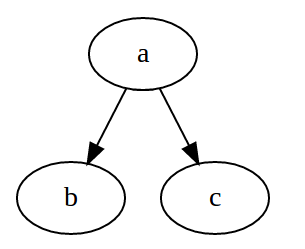
\includegraphics[width=8cm]{bilder/graphVizExample.png}
\caption{Generated graph image from Listing \ref{vizJs}.}
\label{graphVizEx}
\end{figure}
\end{center}